\chapter{Analyse}

\section{Analyse de la relaxation}
\graphicspath{{04-Analyse/}}
\minitoc
Le processus de relaxation utilisé dans l'algorithme CxSOM est une méthode originale pour construire des connexions bidirectionnelles entre cartes. Deux cartes connectées de cette façon jouent alors un rôle symétrique, contrairement à une connexion unidirectionnelle ou hiérafchique ou une carte joue le rôle d'entrée. Dans cette section, nous évaluons expérimentalement la méthode de relaxation en tant que moyen de trouver une Best Matching Unit cohérente. On cherchera notamment à répondre aux questions suivantes :  
\begin{itemize}
\item Est-ce que la méthode de relaxation converge ?
\item Est-ce que que cette méthode est déterministe ?
\item Quels sont les paramètres à prendre en compte dans l'algorithme de relaxation ?
\end{itemize}

\subsection{Formalisation Mathématique de la relaxation}
La relaxation est une recherche de point fixe de l'activité globale de chaque carte de l'architecture. L'équation suivante décrit le processus de relaxation. 
\begin{equation}
\text{Pour toute carte $i$}, \bmu\m{i}_{\tau +1} = f\m{i}(\bmu\m{0}_\tau,\cdots,\bmu\m{N}_\tau)
\label{eq:evolution}
\end{equation}
avec
\begin{equation}
\begin{split}
\forall i, &f\m{i}(\bmu\m{0},\cdots,\bmu\m{N})= \bmu\m{i}_{\tau} \pm \min(\delta, \lvert \bmu\m{i}_{\tau} - \argmax_{p\m{i}}(a_g(p\m{i},\bmu\m{i_0}_\tau, \cdots \bmu\m{i_K}_\tau) \rvert),\\
&i_0, \cdots i_K \; \text{indices des cartes nourrissant la carte $i$}.
\end{split}
\label{eq:fonction}
\end{equation}
Il s'agit d'une suite récurrente définie par $\mathbf{\bmu}_{\tau+1} = \mathbf{f}(\mathbf{\bmu}_\tau)$.
Dans l'algorithme CxSOM,$(\bmu\m{0}_0, \cdots , \bmu\m{N}_0)$ est défini dans chaque carte à : 
\begin{equation}
\begin{cases}
\bmu\m{0} = \argmax_{p\m{0}} a_e(p\m{0},\inpx\m{0})\\
\cdots \\
\bmu\m{N} = \argmax_{p\m{N}} a_e(p\m{N},\inpx\m{N})\\
\end{cases}
\label{eq:init}
\end{equation}

La relaxation se traduit par une recherche de point fixe de la suite $\mathbf{\bmu_{\tau+1}} = \mathbf{\bmu_{\tau}}$, soit:
\begin{equation}
\mathbf{\bmu} = \mathbf{f}(\mathbf{\bmu})
\label{eq:suite}
\end{equation}

Si $f$ admet un point fixe, alors ce point fixe est aussi un point fixe pour la suite $\mathbf{\bmu}_\tau$. Pour s'assurer de la convergence de l'algorithme de relaxation, il faut aussi vérifier que:
\begin{itemize}
\item Le point fixe de $f$ est unique.
\item $\mathbf{\bmu_\tau}$ converge
\end{itemize}

Expérimentalement, il semble que si $\mathbf{f}$ admet un unique point fixe, alors $\mathbf{\bmu_\tau}$ converge vers ce point fixe. On montrera que ce point fixe n'est pas toujours unique, notamment lorsque les poids sont aléatoires au début de l'apprentissage, ce qui entraîne alors une non-convergence de la relaxation. Cependant, ces cas n'influencent pas l'apprentissage des cartes en choissant des bons paramètres d'apprentissage. On observera expérimentalement qu'à la fin de l'apprentissage, la disposition des poids permet l'existence d'un unique point fixe. 

\subsection{Méthodes et Résultats}

\subsubsection{Etude de la convergence des BMUs lors de la relaxation}

La méthode de relaxation cherche la convergence des BMUs de l'architectures. Nous avons donc réalisé 1000 itérations de test, à poids figés, à différents temps d'apprentissage, et comptons le nombre de pas nécessaires à la convergence de la relaxation. L'algorithme utilisé pour la relaxation s'arrête automatiquement si la relaxation dépasse 1000 itérations. On considérera que la relaxation n'a pas atteint un point de convergence si la relaxation atteint ces 1000 itérations.
Plusieurs situations amènent à une non-convergence des cartes  : 
\begin{itemize}
\item La relaxation évolue vers un point de convergence, mais trop lentement pour y arriver en moins de 1000 itérations
\item La relaxation évolue vers un cycle limite composé d'un nombre limité d'unités étant alternativement best matching units
\item La relaxation évolue sans répétition de motifs dans la carte : évolution chaotique.
\end{itemize}
Le premier cas est évité en prenant la limite du nombre d'itérations possible assez grande par rapport à la taille de la carte, en l'occurence 1000 alors que les cartes sont de tailles 500. Le pas d'évolution de la relaxation est d'une dizaine d'unités. La convergence, si elle existe, est donc rapide.

L'étude de la convergence sera réalisée dans des architectures de 2 et 3 cartes, pour des cartes une dimension et deux dimensions.

\begin{figure}
\centering
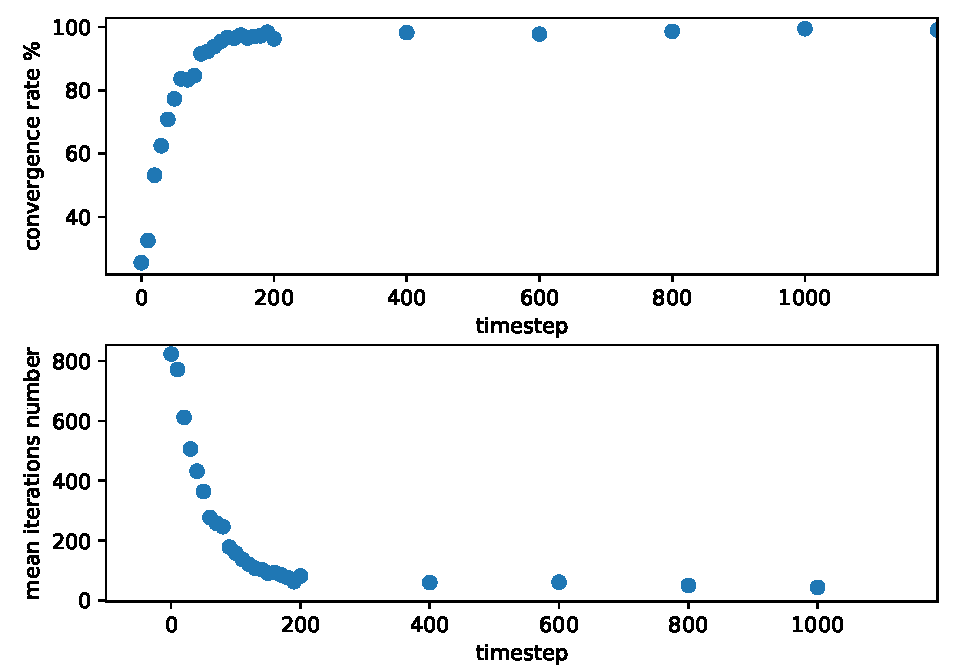
\includegraphics[width=0.8\textwidth]{1D_conv_evolution.pdf}
\caption{Evolution du taux de convergence lors de la relaxation au cours de l'apprentissage sur deux cartes 1D. Chaque point est calculé sur un échantillon de 1000 relaxations au temps t, évaluées sur des entrées différentes prises aléatoirement sur le cercle.}
\label{fig:conv_evolution}
\end{figure}


\begin{figure}
\centering
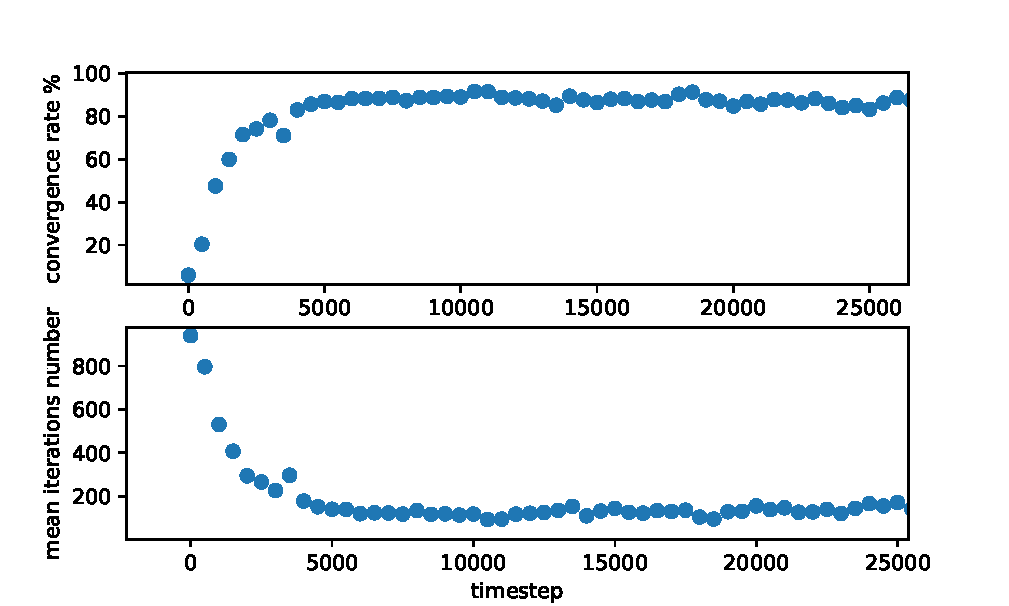
\includegraphics[width=0.8\textwidth]{2D_conv_evolution.pdf}
\caption{Evolution du taux de convergence lors de la relaxation au cours de l'apprentissage sur deux cartes 2D. Chaque point est calculé sur un échantillon de 1000 relaxations au temps t, évaluées sur des entrées différentes prises aléatoirement sur le cercle.}
\label{fig:conv_evolution}
\end{figure}

\subsubsection{Etude de l'influence de l'entrée contextuelle sur le BMU}

Selon l'équation \ref{eq:suite}, l'évolution de la suite $\mathbf{\bmu_tau}$ dépend d'une fonction $\mathbf{f}$ ne dépendant pas de $\tau$. Dans le cas d'une architecture de deux cartes $M\m{1}$ et $M\m{2}$ prenant en entrée respectivement $\inpx\m{1} = X, \inpx\m{2} = Y$, cette évolution peut être réécrite en:
\begin{equation}
\begin{cases}
\bmu\m{1}_{\tau+1} = 
\end{cases}
\end{equation}

Les BMUS prenant des valeurs discrètes, il est possible de calculer le tableau de valeurs de $\mathbf{f}(\bmu\m{1},\bmu\m{2})$ et de le représenter en deux dimensions. Cela permet alors d'évualer la contribution des entrées contextuelles dans le calcul de $\bmu$.

\begin{figure}
\centering
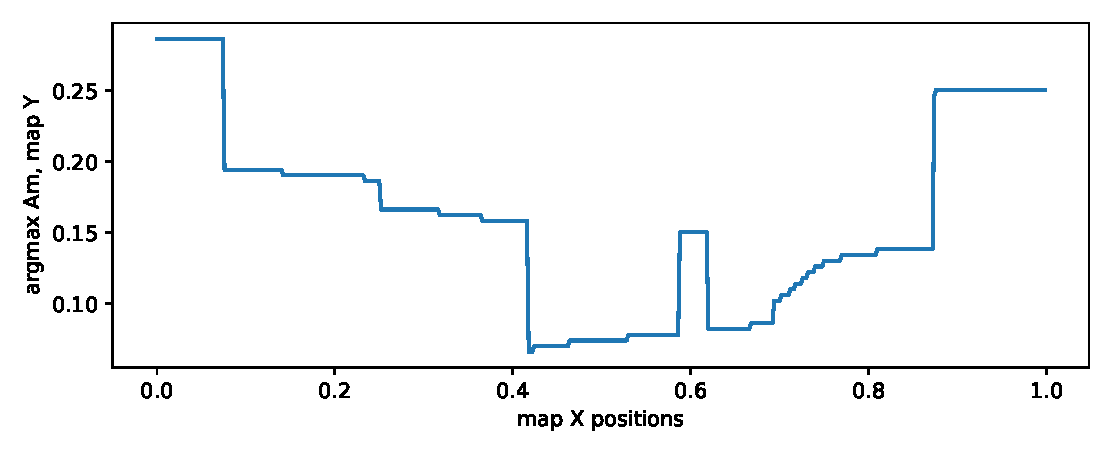
\includegraphics[width=0.7\textwidth]{am_006_X.pdf}
\end{figure}

\begin{figure}
\centering
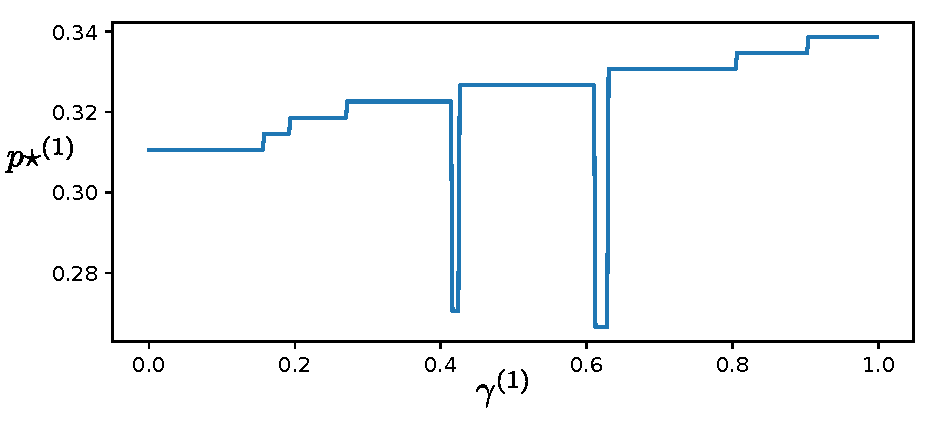
\includegraphics[width=0.7\textwidth]{am_006.pdf}
\end{figure}

\subsubsection{Etude de l'unicité du point fixe}

On étudiera donc l'évolution de processus de relaxation lancés sur les mêmes poids, pour une entrée externe fixée, intialisés à des valeurs aléatoires de BMU dans chaque carte.
Chacun de ces processus aboutit sur un point de convergence; on tracera donc la distance moyenne entre les différents points de convergence sur toutes les expériences. Si cette distance est nulle, alors le point de convergence est un point fixe qui ne dépend pas de l'initialisation. 
Cette étude sera réalisée sur des cartes 1D et 2D, pour des architectures de 2 et trois cartes.

\begin{figure}
\begin{minipage}{0.5\textwidth}
\centering
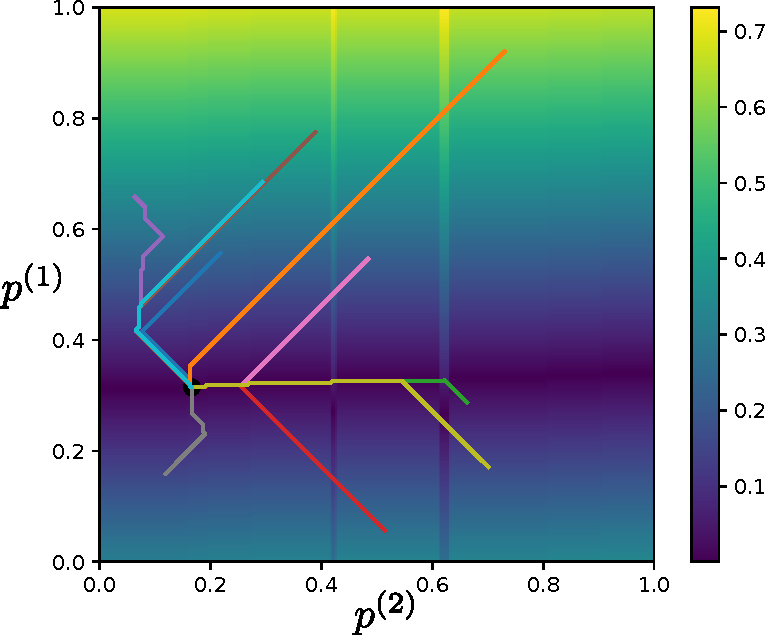
\includegraphics[width=\textwidth]{champ_X_006.pdf}
\end{minipage}
\begin{minipage}{0.5\textwidth}
\centering
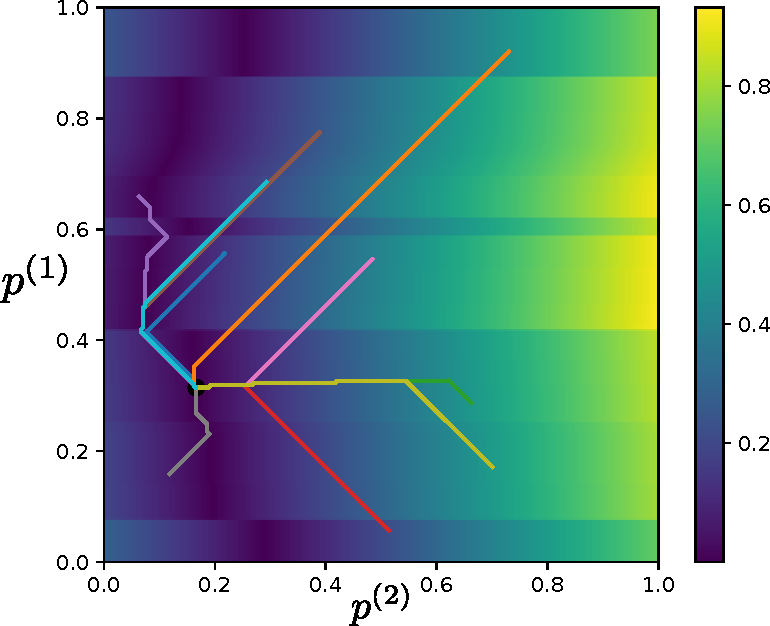
\includegraphics[width=\textwidth]{champ_Y_006.pdf}
\end{minipage}
\caption{Valeur de $p\star\m{1} - p\m{1}$, resp. $p\star\m{2} - p\m{2}$. $p\star\m{1}$ ne dépend que de $p\m{2}$ : on peut donc tracer cette valeur selon deux dimensions pour chaque carte. Les zones où cette valeur est nulle sont en violet sur le graphique. Les points fixes, s'il existent, sont aux positions de différence nulle pour $M\m{1}$ et $M\m{2}$.}
\label{fig:diff_relax}
\end{figure}

\begin{figure}
\begin{minipage}{0.5\textwidth}
\centering
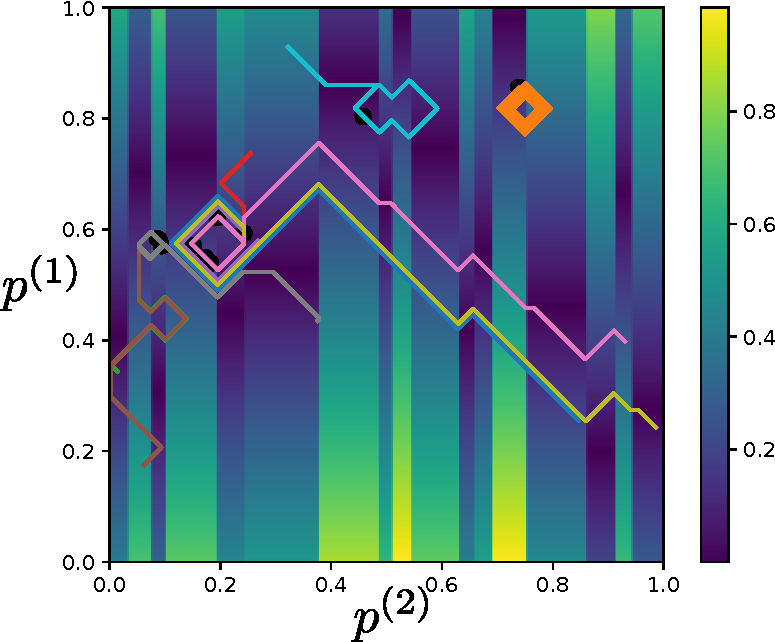
\includegraphics[width=\textwidth]{champ_X_006_t1.pdf}
\end{minipage}
\begin{minipage}{0.5\textwidth}
\centering
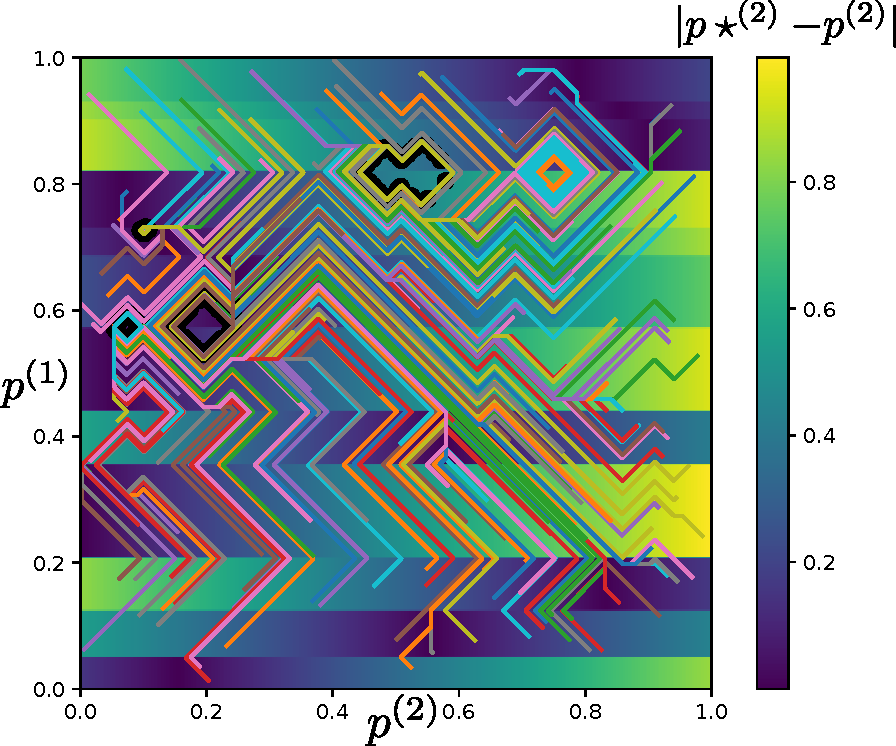
\includegraphics[width=\textwidth]{champ_Y_006_t1.pdf}
\end{minipage}
\caption{Valeur de $p\star\m{1} - p\m{1}$, resp. $p\star\m{2} - p\m{2}$. $p\star\m{1}$ ne dépend que de $p\m{2}$ : on peut donc tracer cette valeur selon deux dimensions pour chaque carte. Les zones où cette valeur est nulle sont en violet sur le graphique. Les points fixes, s'il existent, sont aux positions de différence nulle pour $M\m{1}$ et $M\m{2}$.}
\label{fig:diff_relax_t1}
\end{figure}

\begin{figure}
\centering
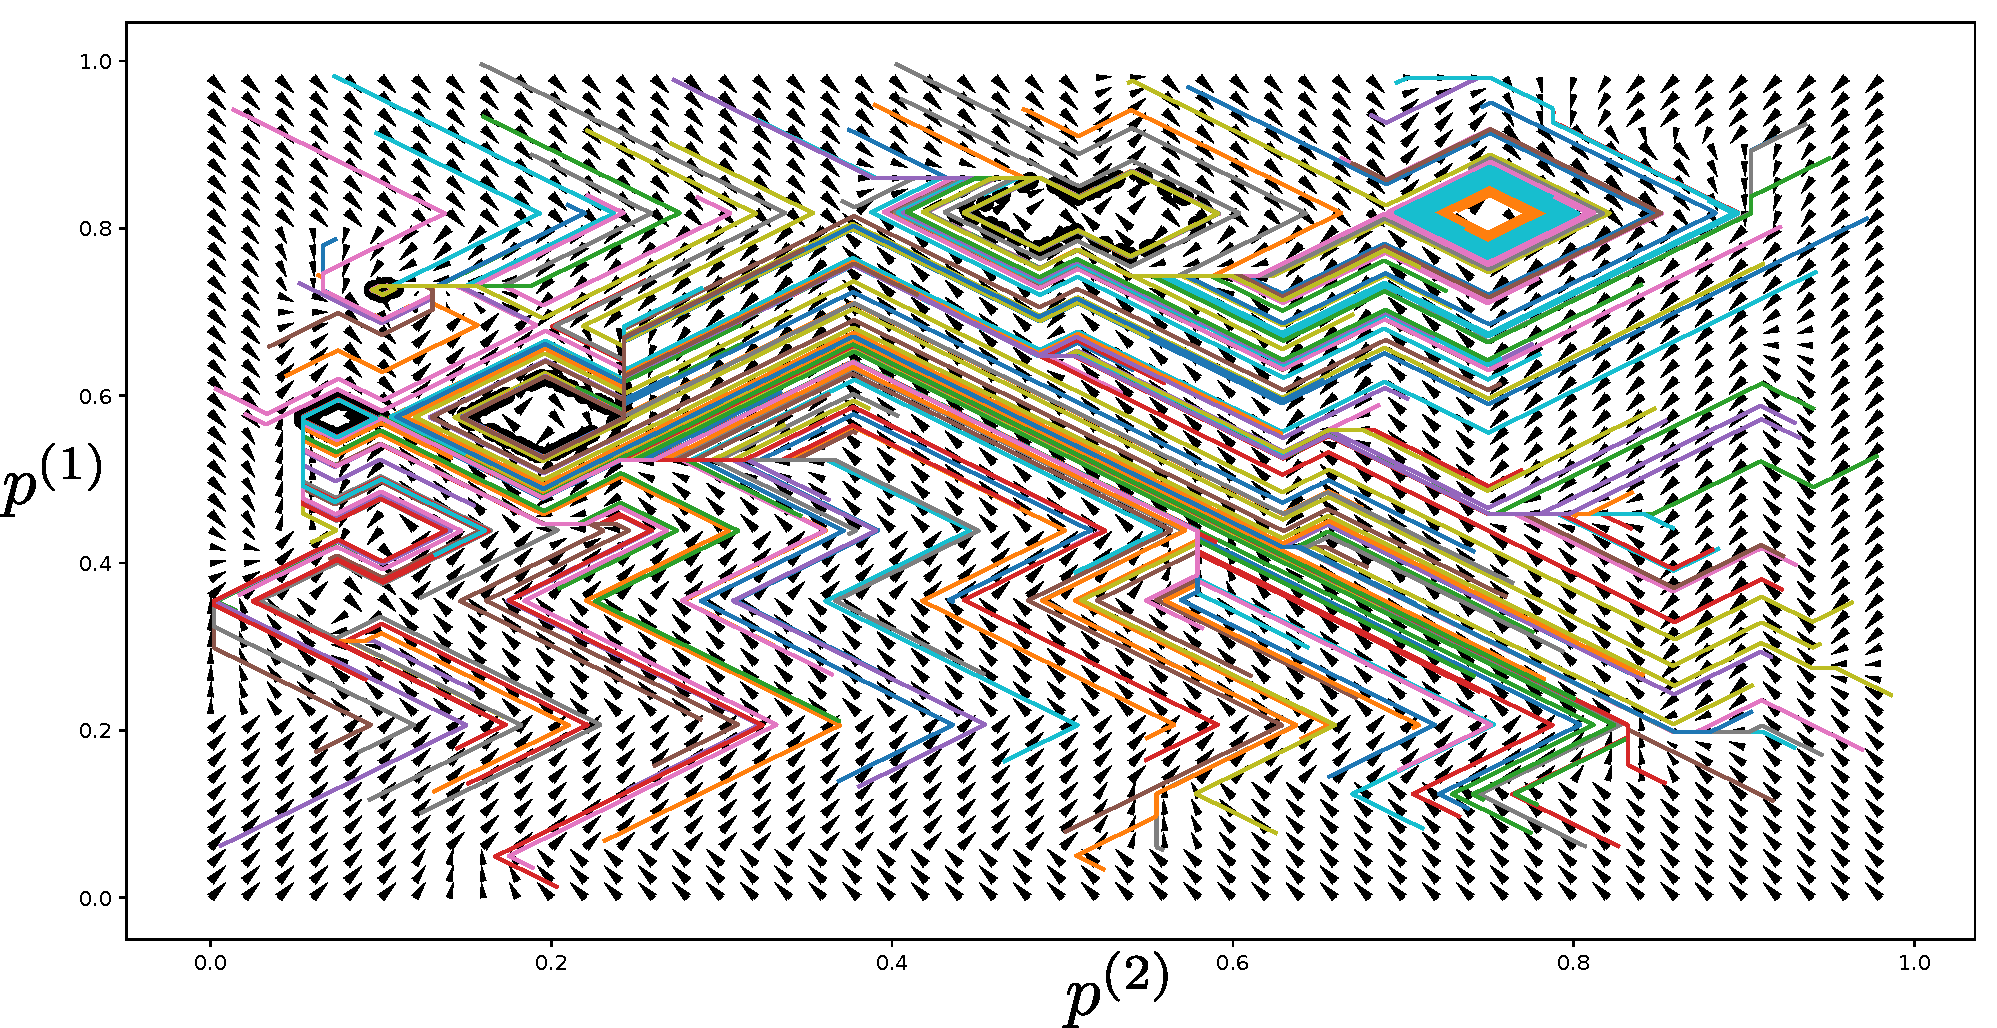
\includegraphics[width=\textwidth]{champ_006_t1.pdf}
\end{figure}


\begin{figure}
\centering
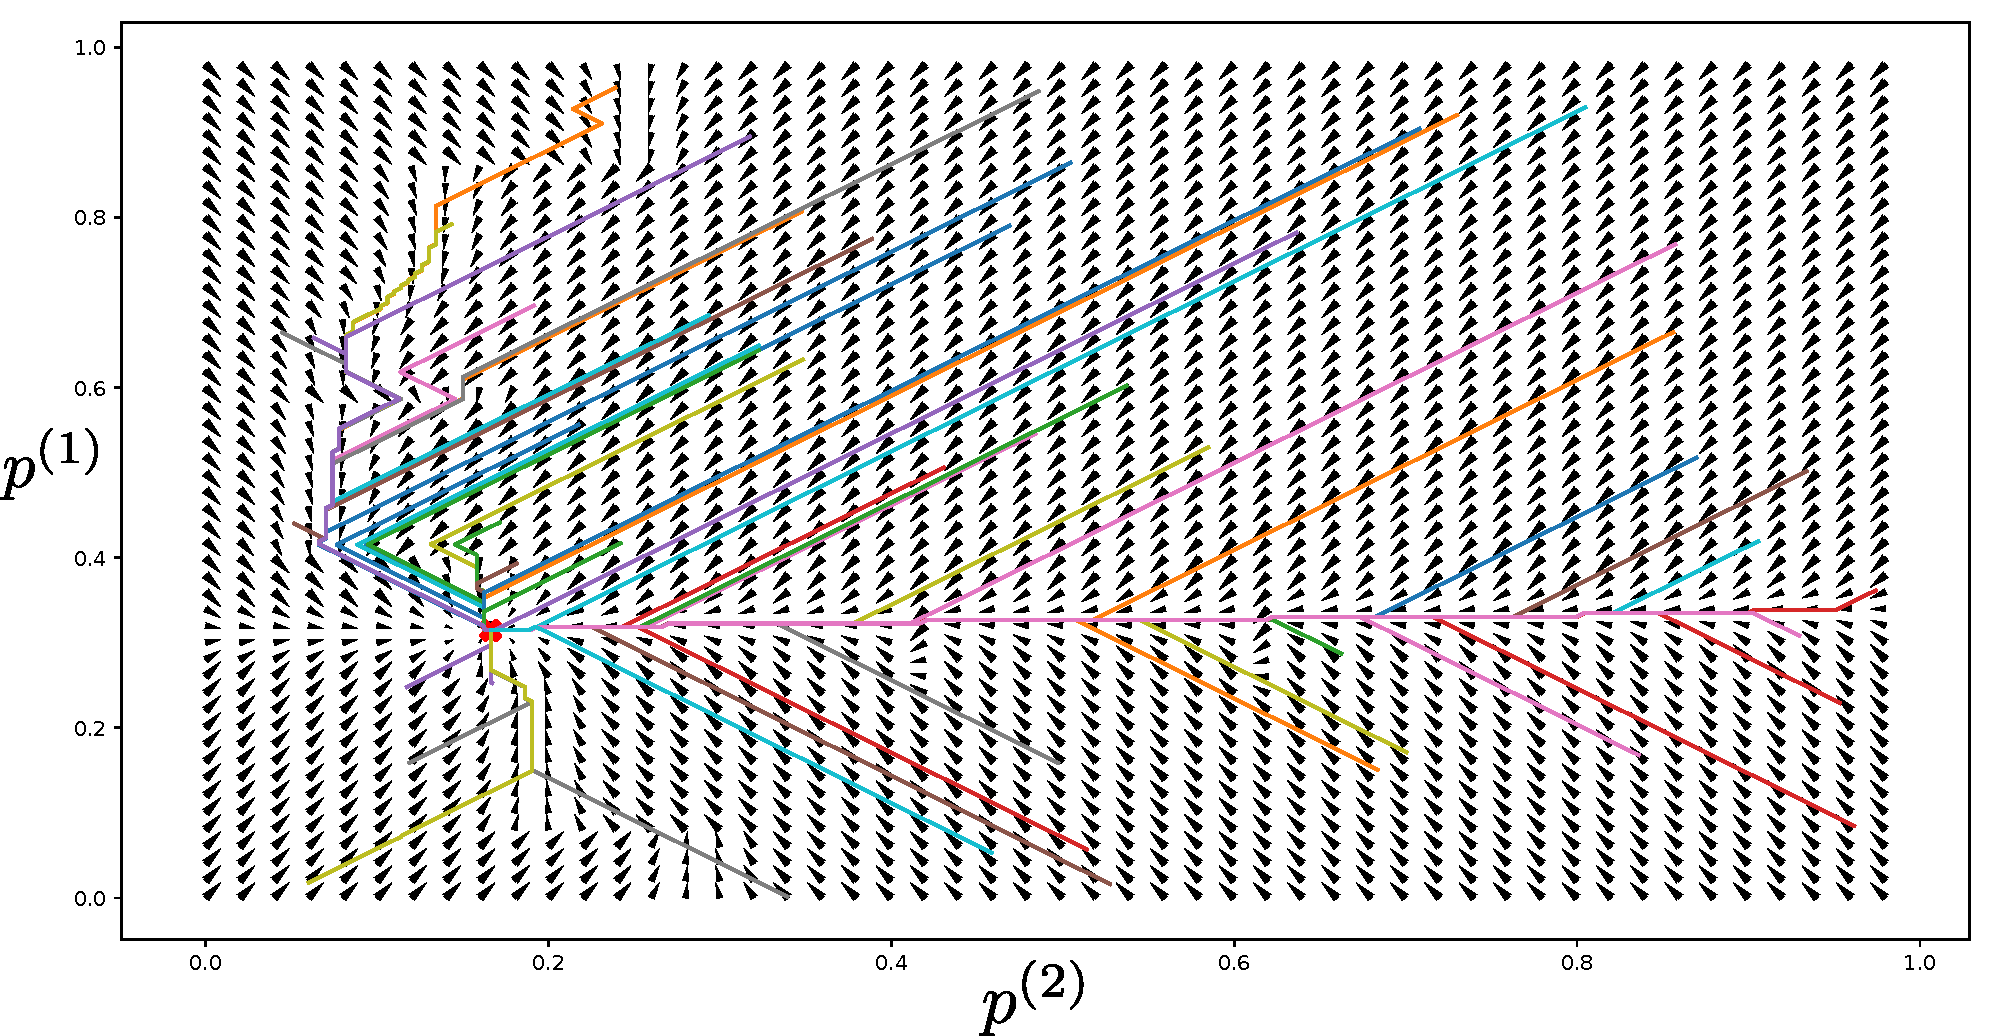
\includegraphics[width=\textwidth]{champ_006.pdf}
\end{figure}
\subsection{Résultats}

\subsection{Discussion}

\draft{
\begin{itemize}
\item Element clé de l'architecture : relaxation. A t-on toujours un point de convergence ? Sinon, dans quels cas ? 
\item On peut tracer les champs de relaxation pour trouver le point fixe. 
\item Une carte est un système dynamique comme une variable passant d'un état à un autre. Etat = BMU.
\end{itemize}
}


\section{Analyse de l'auto-organisation}